% This file was converted to LaTeX by Writer2LaTeX ver. 1.0.2
% see http://writer2latex.sourceforge.net for more info
\documentclass[a4paper]{book}
\usepackage[utf8]{inputenc}
\usepackage[T1]{fontenc}
\usepackage[french]{babel}
\usepackage{amsmath}
\usepackage{textcomp}
\usepackage{amssymb,amsfonts,textcomp}
\usepackage{color}
\usepackage{array}
\usepackage{hhline}
\usepackage{hyperref}
\hypersetup{pdftex, colorlinks=true, linkcolor=blue, citecolor=blue, filecolor=blue, urlcolor=blue, pdftitle=, pdfauthor=, pdfsubject=, pdfkeywords=}
\usepackage[pdftex]{graphicx}
% Outline numbering
\setcounter{secnumdepth}{2}
\renewcommand\thesection{\Roman{section}}
\renewcommand\thesection{\arabic{section}}
% Page layout (geometry)
\setlength\voffset{-1in}
\setlength\hoffset{-1in}
\setlength\topmargin{2cm}
\setlength\oddsidemargin{2cm}
\setlength\textheight{25.7cm}
\setlength\textwidth{17.001cm}
\setlength\footskip{0.0cm}
\setlength\headheight{0cm}
\setlength\headsep{0cm}
% Footnote rule
\setlength{\skip\footins}{0.119cm}
\renewcommand\footnoterule{\vspace*{-0.018cm}\setlength\leftskip{0pt}\setlength\rightskip{0pt plus 1fil}\noindent\textcolor{black}{\rule{0.25\columnwidth}{0.018cm}}\vspace*{0.101cm}}
% Pages styles
\makeatletter
\newcommand\ps@Standard{
  \renewcommand\@oddhead{}
  \renewcommand\@evenhead{}
  \renewcommand\@oddfoot{}
  \renewcommand\@evenfoot{}
  \renewcommand\thepage{\arabic{page}}
}
\newcommand\ps@RightPage{
  \renewcommand\@oddhead{}
  \renewcommand\@evenhead{}
  \renewcommand\@oddfoot{}
  \renewcommand\@evenfoot{}
  \renewcommand\thepage{\arabic{page}}
}
\newcommand\ps@LeftPage{
  \renewcommand\@oddhead{}
  \renewcommand\@evenhead{}
  \renewcommand\@oddfoot{}
  \renewcommand\@evenfoot{}
  \renewcommand\thepage{\arabic{page}}
}
\makeatother
\thispagestyle{Standard}
\title{}
\author{}
\date{2018-07-26T17:55:01.714755971}
\begin{document}
\clearpage\setcounter{page}{1}\pagestyle{LeftPage}
\thispagestyle{RightPage}

{\centering\sffamily\bfseries
LE BLUES \par
Documents supports
\par}

{\centering\sffamily\bfseries
M\'ethodes de Guitare, Basse, Contrebasse,Blues.
\par}


{\centering\sffamily\bfseries
(plus quelques autres styles jazz, rock, jazz-rock, latin)
\par}

{\centering
DD externe Samsung
\par}

{\centering
Lenovo
\par}

\setcounter{tocdepth}{10}
\renewcommand\contentsname{Table des mati\`eres}
\tableofcontents



\clearpage

\part{Méthodes instrumentales}
\chapter{Méthodes de guitare}




\clearpage\section[200 acoustick
liks]{200 acoustick liks}
\hypertarget{RefHeadingToc102973218262}{}

\begin{center}
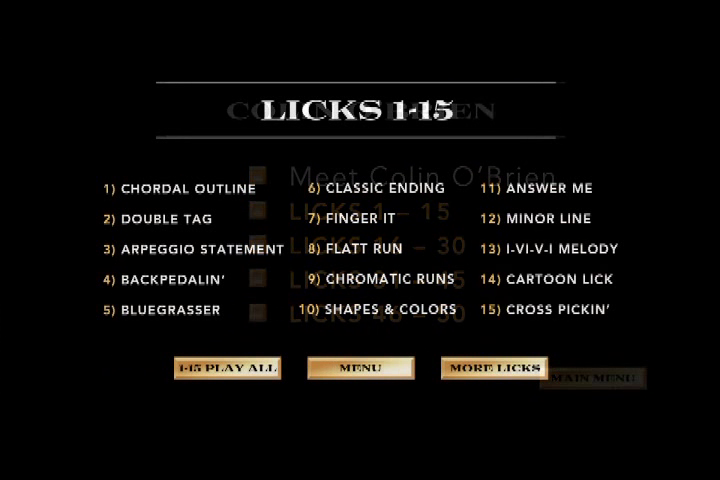
\includegraphics[width=17cm,height=11.333cm]{lebluessupportsmethodes-img1.png}
\end{center}


\begin{center}
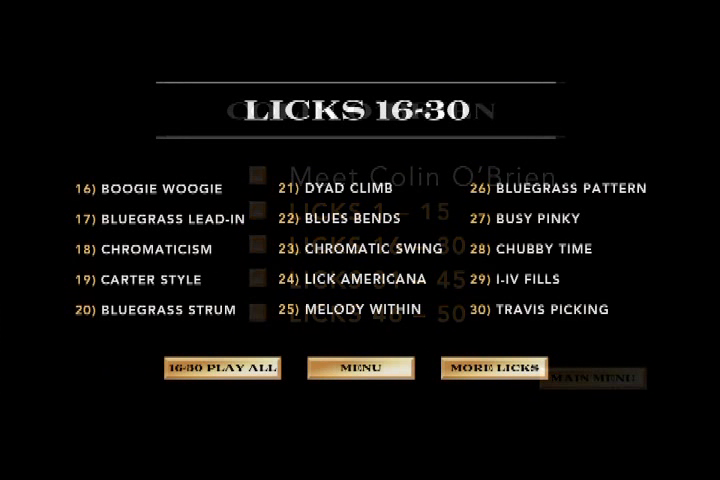
\includegraphics[width=17cm,height=11.333cm]{lebluessupportsmethodes-img2.png}
\end{center}


\begin{center}
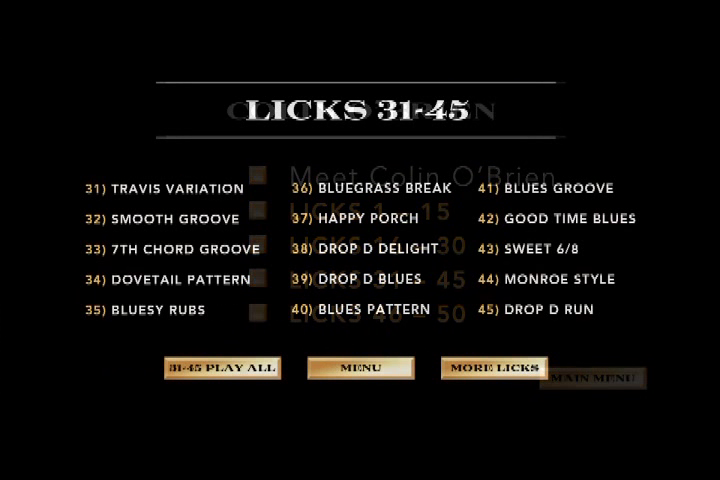
\includegraphics[width=17cm,height=11.333cm]{lebluessupportsmethodes-img3.png}
\end{center}


\begin{center}
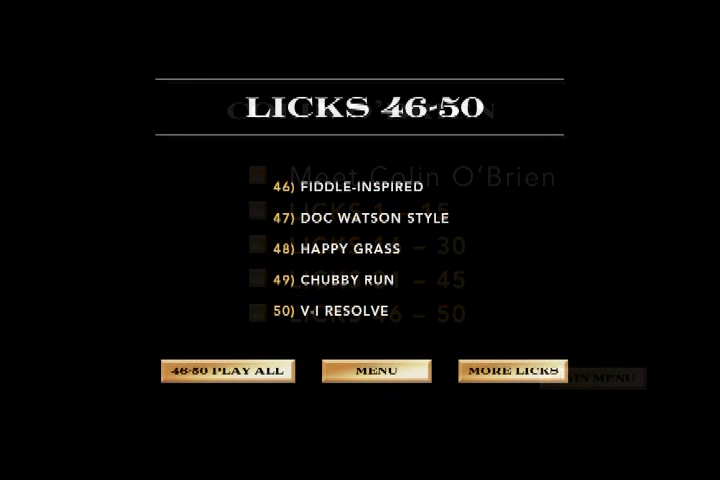
\includegraphics[width=17cm,height=11.333cm]{lebluessupportsmethodes-img4.png}
\end{center}
\clearpage

\begin{center}
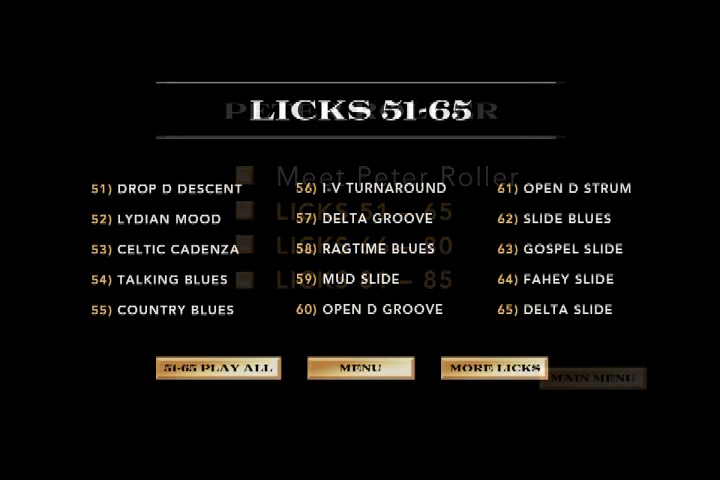
\includegraphics[width=17cm,height=11.333cm]{lebluessupportsmethodes-img5.png}
\end{center}


\begin{center}
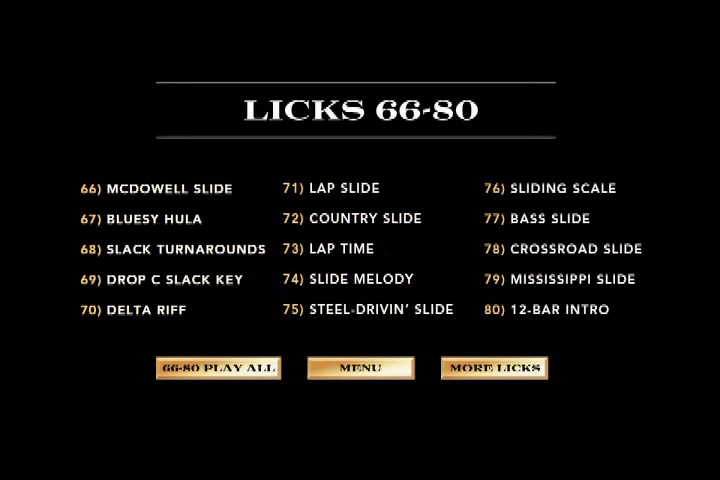
\includegraphics[width=17cm,height=11.333cm]{lebluessupportsmethodes-img6.png}
\end{center}



\clearpage

\begin{center}
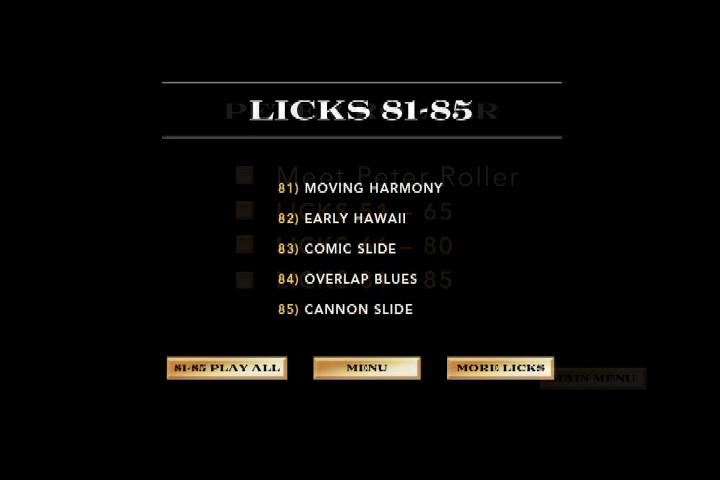
\includegraphics[width=17cm,height=11.333cm]{lebluessupportsmethodes-img7.png}
\end{center}


\begin{center}
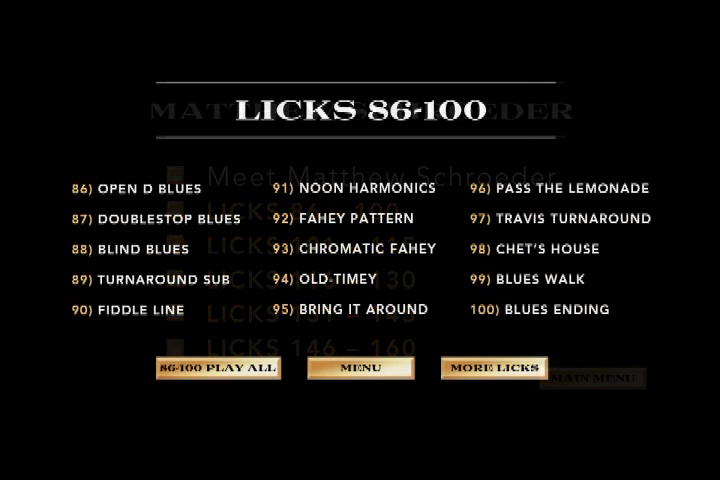
\includegraphics[width=17cm,height=11.333cm]{lebluessupportsmethodes-img8.png}
\end{center}



\clearpage

\begin{center}
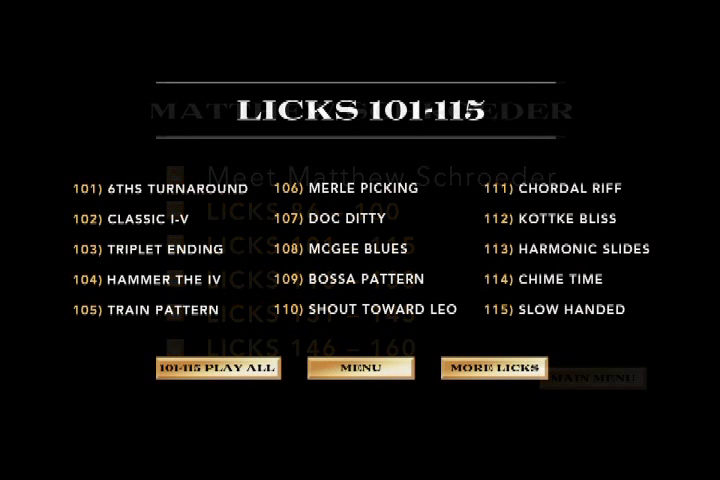
\includegraphics[width=17cm,height=11.333cm]{lebluessupportsmethodes-img9.png}
\end{center}





\begin{center}
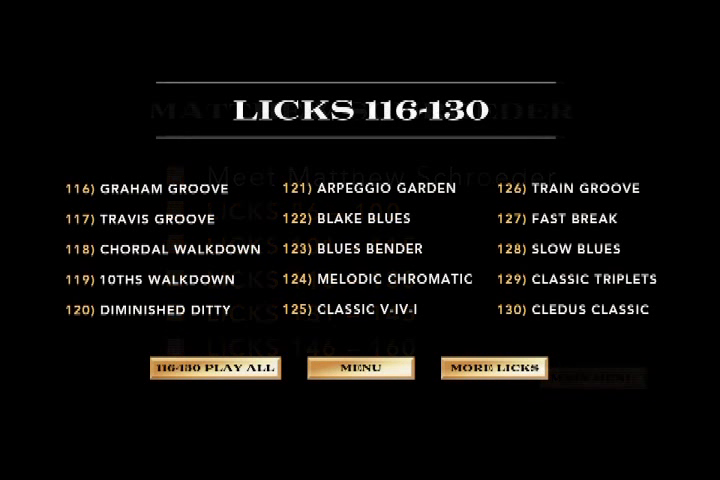
\includegraphics[width=17cm,height=11.333cm]{lebluessupportsmethodes-img10.png}
\end{center}
\clearpage

\begin{center}
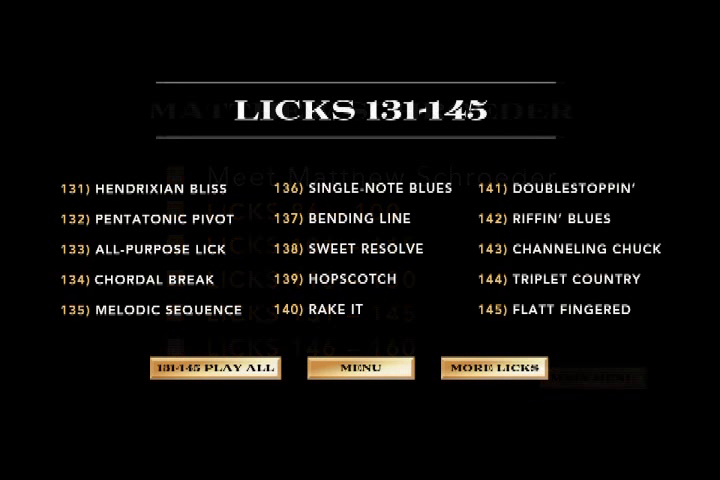
\includegraphics[width=17cm,height=11.333cm]{lebluessupportsmethodes-img11.png}
\end{center}





\begin{center}
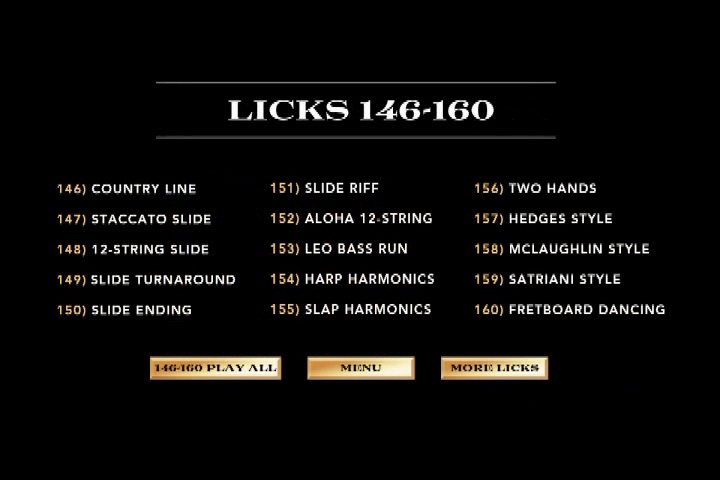
\includegraphics[width=17cm,height=11.333cm]{lebluessupportsmethodes-img12.png}
\end{center}



\clearpage

\begin{center}
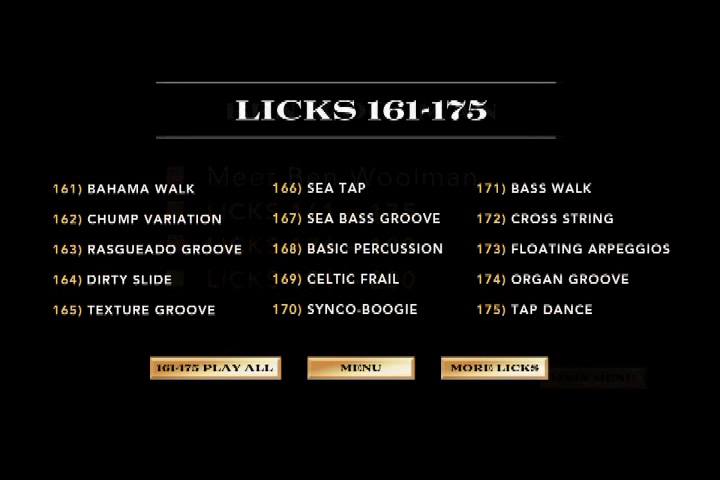
\includegraphics[width=17cm,height=11.333cm]{lebluessupportsmethodes-img13.png}
\end{center}


\begin{center}
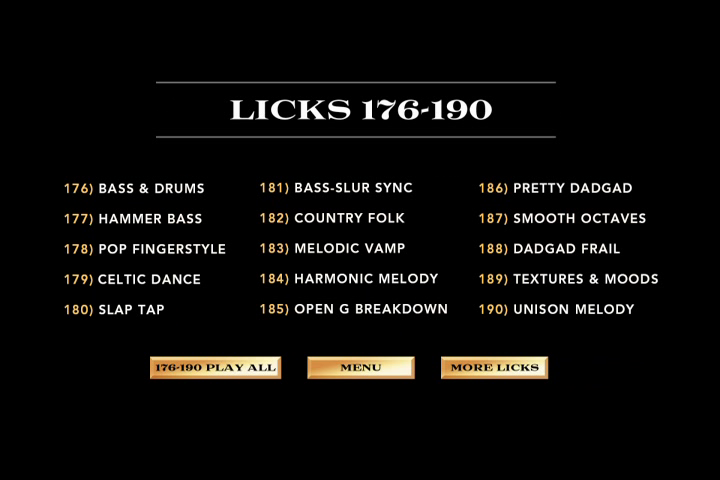
\includegraphics[width=17cm,height=11.333cm]{lebluessupportsmethodes-img14.png}
\end{center}



\clearpage

\begin{center}
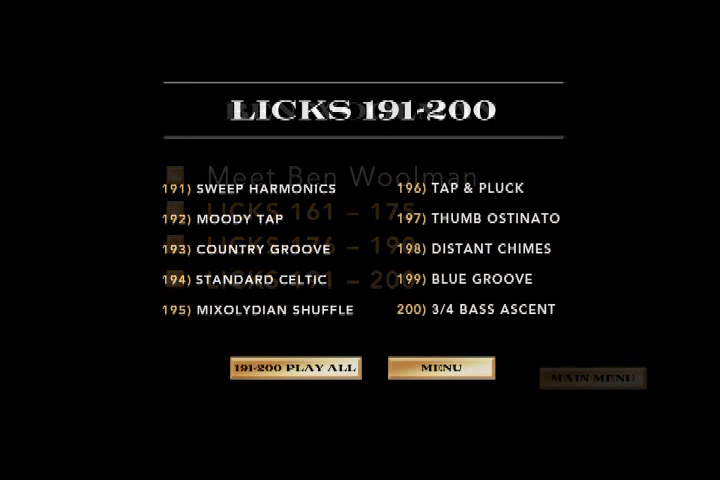
\includegraphics[width=17cm,height=11.333cm]{lebluessupportsmethodes-img15.png}
\end{center}
\clearpage\section[200 blues licks]{200 blues licks}
\hypertarget{RefHeadingToc104973218262}{}

\begin{center}
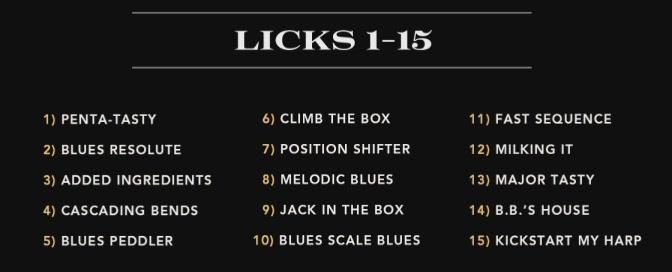
\includegraphics[width=17cm,height=6.881cm]{lebluessupportsmethodes-img16.jpg}
\end{center}
\begin{center}
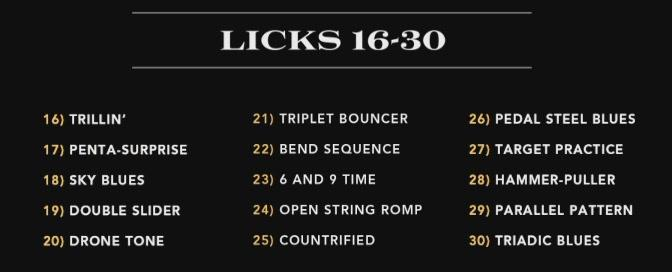
\includegraphics[width=17cm,height=6.881cm]{lebluessupportsmethodes-img17.jpg}
\end{center}


\begin{center}
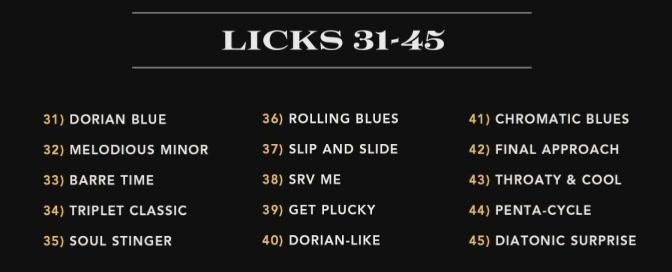
\includegraphics[width=17cm,height=6.881cm]{lebluessupportsmethodes-img18.jpg}
\end{center}



\clearpage







\begin{center}
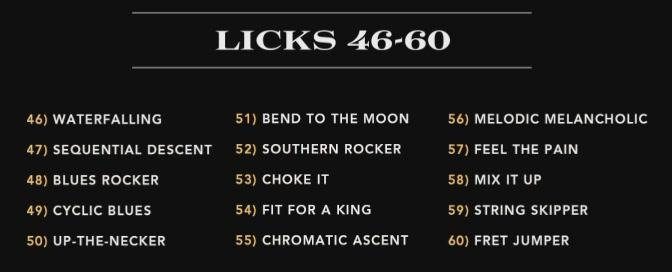
\includegraphics[width=17cm,height=6.881cm]{lebluessupportsmethodes-img19.jpg}
\end{center}


\begin{center}
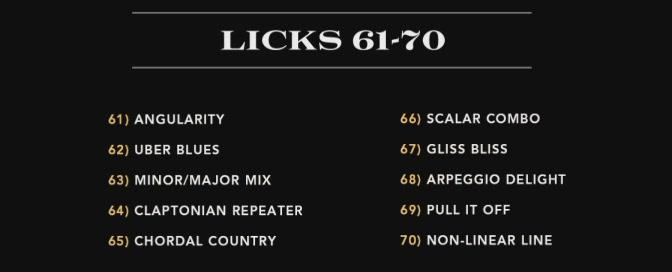
\includegraphics[width=17cm,height=6.881cm]{lebluessupportsmethodes-img20.jpg}
\end{center}


\begin{center}
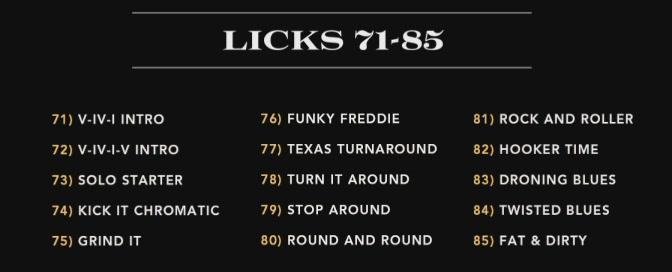
\includegraphics[width=17cm,height=6.881cm]{lebluessupportsmethodes-img21.jpg}
\end{center}



\clearpage

\begin{center}
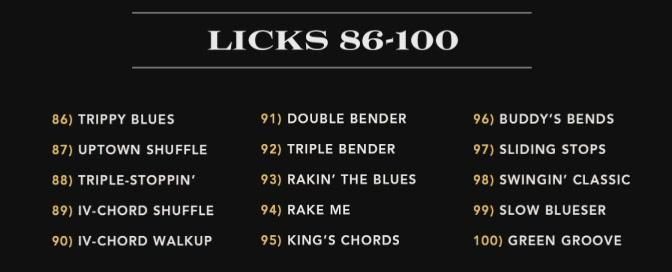
\includegraphics[width=17cm,height=6.881cm]{lebluessupportsmethodes-img22.jpg}
\end{center}


\begin{center}
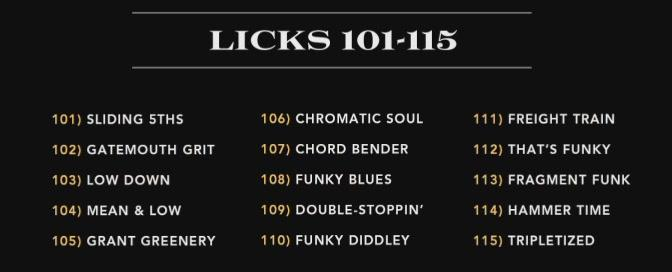
\includegraphics[width=17cm,height=6.881cm]{lebluessupportsmethodes-img23.jpg}
\end{center}


\begin{center}
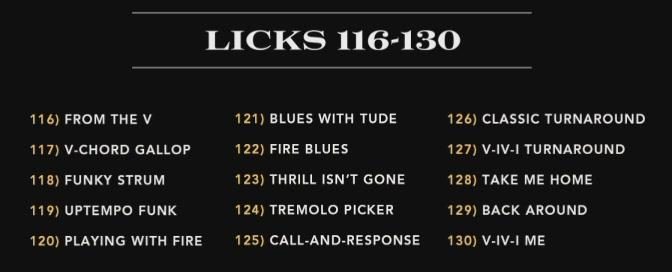
\includegraphics[width=17cm,height=6.881cm]{lebluessupportsmethodes-img24.jpg}
\end{center}



\clearpage

\begin{center}
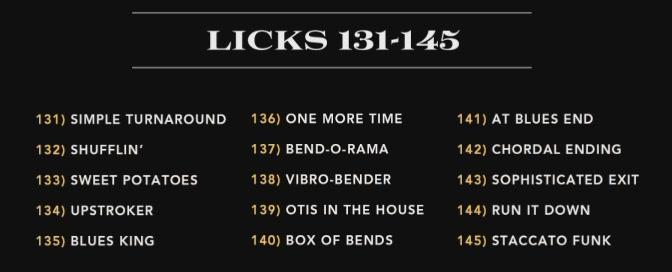
\includegraphics[width=17cm,height=6.881cm]{lebluessupportsmethodes-img25.jpg}
\end{center}


\begin{center}

\includegraphics[width=17cm,height=6.881cm]{lebluessupportsmethodes-img26.jpg}
\end{center}


\begin{center}
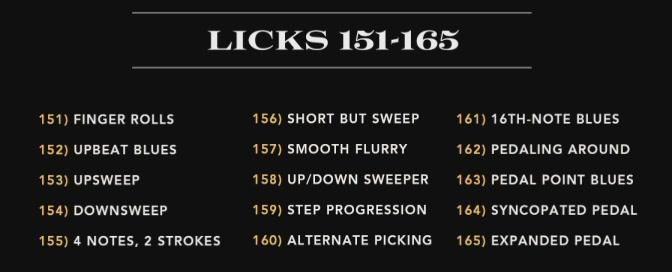
\includegraphics[width=17cm,height=6.881cm]{lebluessupportsmethodes-img27.jpg}
\end{center}






\clearpage

\begin{center}
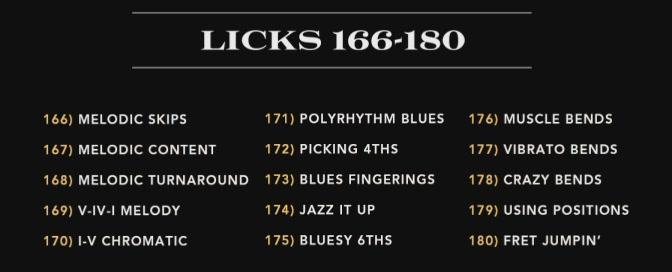
\includegraphics[width=17cm,height=6.881cm]{lebluessupportsmethodes-img28.jpg}
\end{center}


\begin{center}
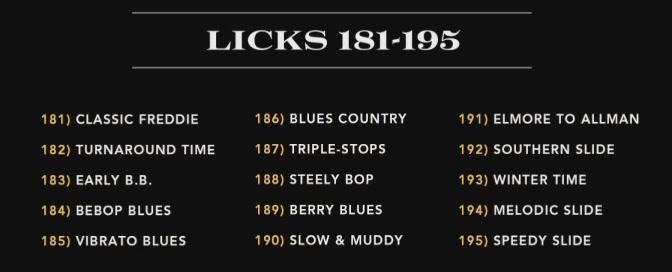
\includegraphics[width=17cm,height=6.881cm]{lebluessupportsmethodes-img29.jpg}
\end{center}


\begin{center}

\includegraphics[width=17cm,height=6.881cm]{lebluessupportsmethodes-img30.jpg}
\end{center}



\clearpage\section[200 jazz licks]{200 jazz licks}
\hypertarget{RefHeadingToc106973218262}{}

\begin{center}
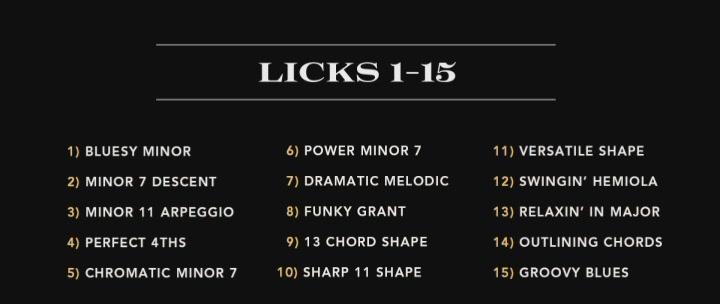
\includegraphics[width=17cm,height=7.177cm]{lebluessupportsmethodes-img31.jpg}
\end{center}


\begin{center}
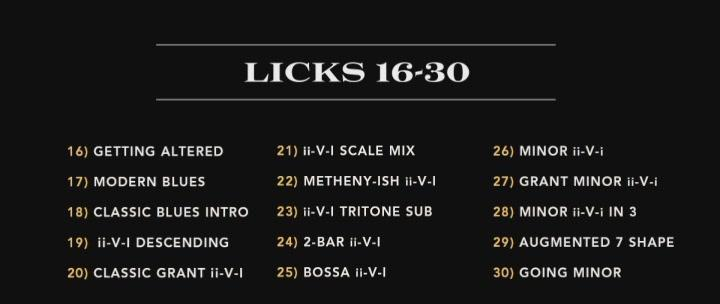
\includegraphics[width=17cm,height=7.177cm]{lebluessupportsmethodes-img32.jpg}
\end{center}


\begin{center}
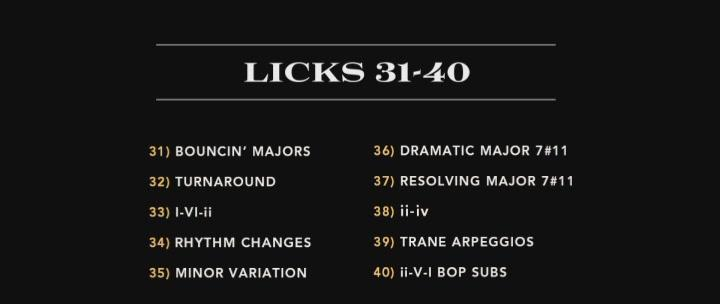
\includegraphics[width=17cm,height=7.177cm]{lebluessupportsmethodes-img33.jpg}
\end{center}
\clearpage

\begin{center}
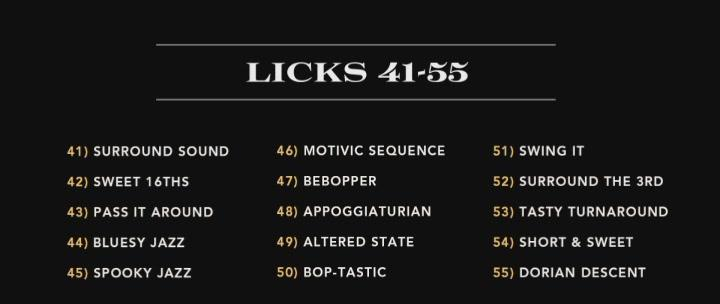
\includegraphics[width=17cm,height=7.177cm]{lebluessupportsmethodes-img34.jpg}
\end{center}


\begin{center}
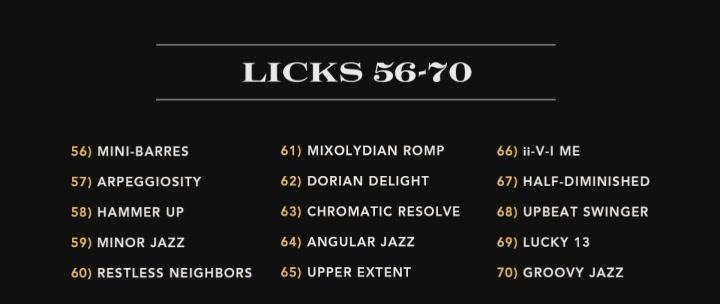
\includegraphics[width=17cm,height=7.177cm]{lebluessupportsmethodes-img35.jpg}
\end{center}


\begin{center}
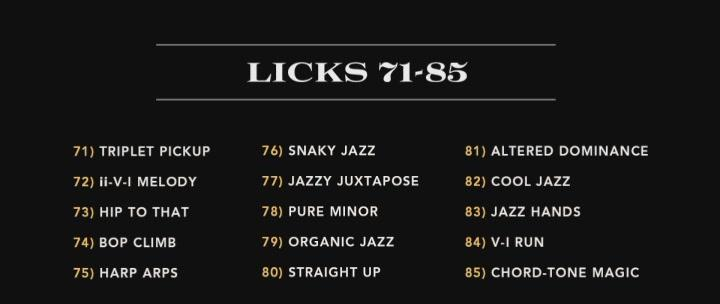
\includegraphics[width=17cm,height=7.177cm]{lebluessupportsmethodes-img36.jpg}
\end{center}



\clearpage

\begin{center}
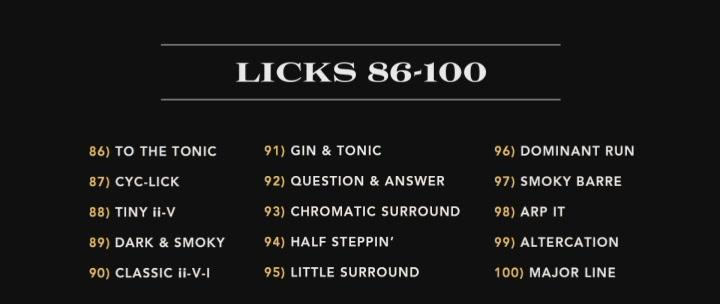
\includegraphics[width=17cm,height=7.177cm]{lebluessupportsmethodes-img37.jpg}
\end{center}


\begin{center}
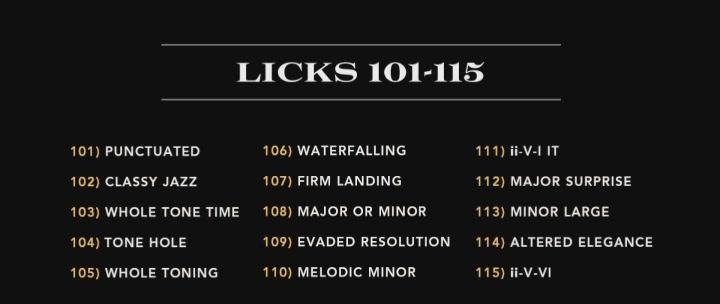
\includegraphics[width=17cm,height=7.177cm]{lebluessupportsmethodes-img38.jpg}
\end{center}


\begin{center}
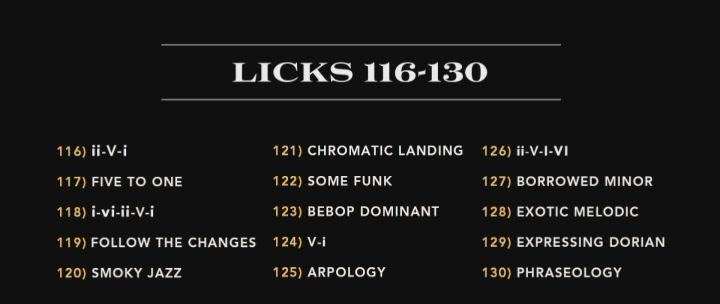
\includegraphics[width=17cm,height=7.177cm]{lebluessupportsmethodes-img39.jpg}
\end{center}



\clearpage

\begin{center}
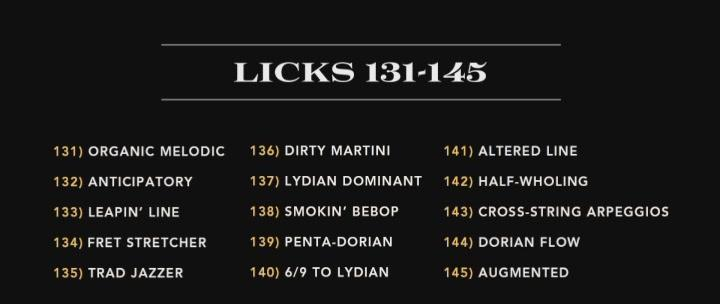
\includegraphics[width=17cm,height=7.177cm]{lebluessupportsmethodes-img40.jpg}
\end{center}


\begin{center}
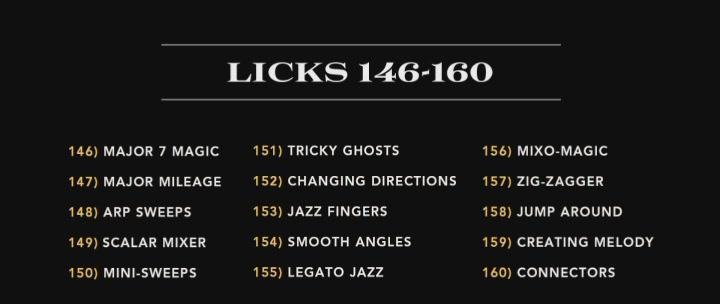
\includegraphics[width=17cm,height=7.177cm]{lebluessupportsmethodes-img41.jpg}
\end{center}


\begin{center}
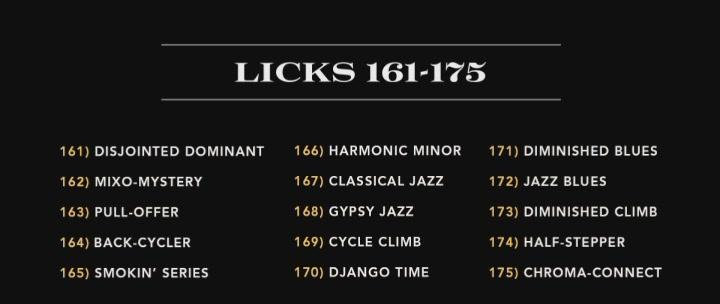
\includegraphics[width=17cm,height=7.177cm]{lebluessupportsmethodes-img42.jpg}
\end{center}



\clearpage

\begin{center}
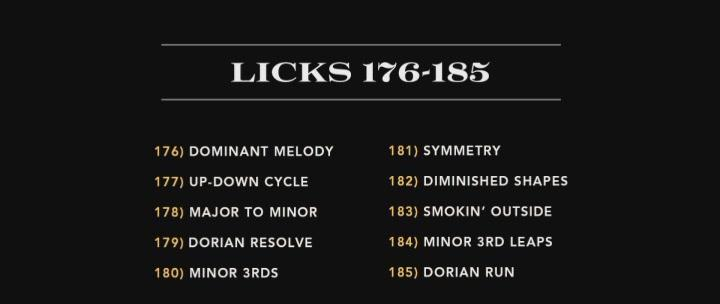
\includegraphics[width=17cm,height=7.177cm]{lebluessupportsmethodes-img43.jpg}
\end{center}


\begin{center}
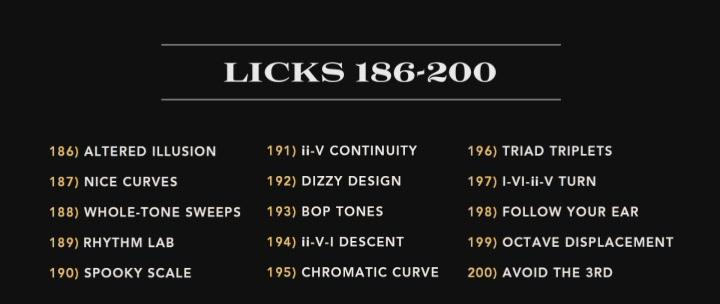
\includegraphics[width=17cm,height=7.177cm]{lebluessupportsmethodes-img44.jpg}
\end{center}
\clearpage\section[Anyone can play jazz guitar]{Anyone can play jazz
guitar}
\hypertarget{RefHeadingToc110973218262}{}1. Jazz. Des gammes.






\begin{center}
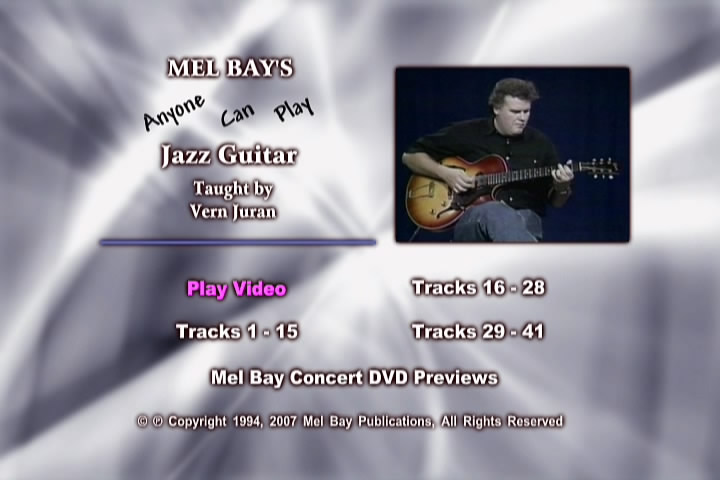
\includegraphics[width=15.023cm,height=10.015cm]{lebluessupportsmethodes-img45.jpg}
\end{center}

\clearpage\section[Art of Acoustic Blues Guitar with Woody Mann/The
Basics]{Art of Acoustic Blues Guitar with Woody Mann/The Basics}
\hypertarget{RefHeadingToc112973218262}{}\ \ Exemple de jeux roots,
Robert Johnson, Charlie Patton etc. Je ne veux pas faire ce style mais
quand m\^eme : 

\ \ 1. 03 One Time Blues.avi bien

\ \ 2. 04 Soo Cow Soo.avi bien

\ \ 3. 05 Pig Meat Strut.avi bien



\begin{center}
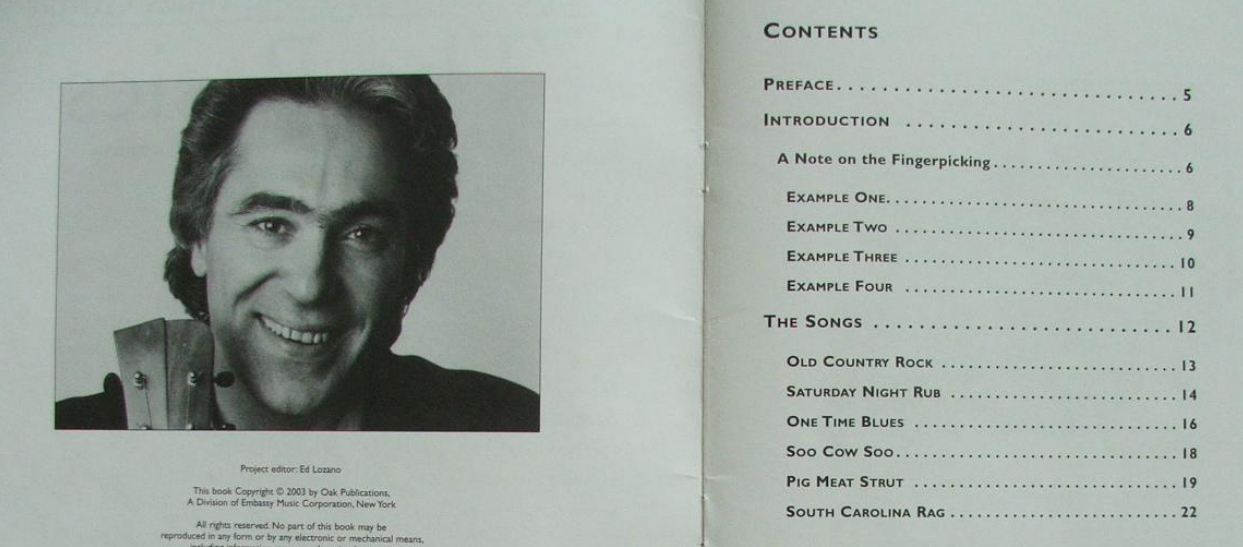
\includegraphics[width=17cm,height=7.479cm]{lebluessupportsmethodes-img46.png}
\end{center}








\begin{center}
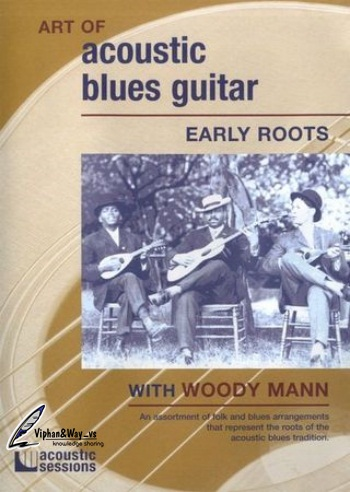
\includegraphics[width=8.64cm,height=12.144cm]{lebluessupportsmethodes-img47.jpg}
\end{center}





\clearpage

\begin{center}
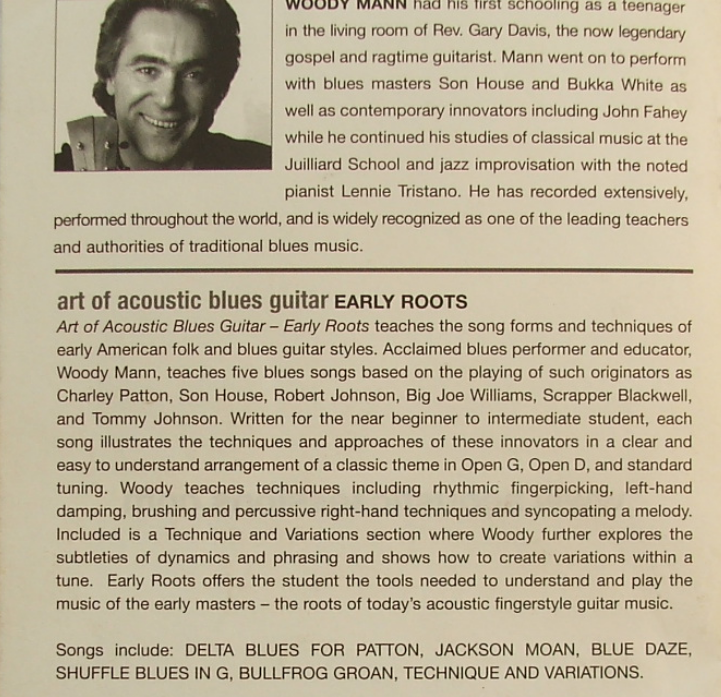
\includegraphics[width=17cm,height=16.434cm]{lebluessupportsmethodes-img48.png}
\end{center}







\clearpage

\begin{center}
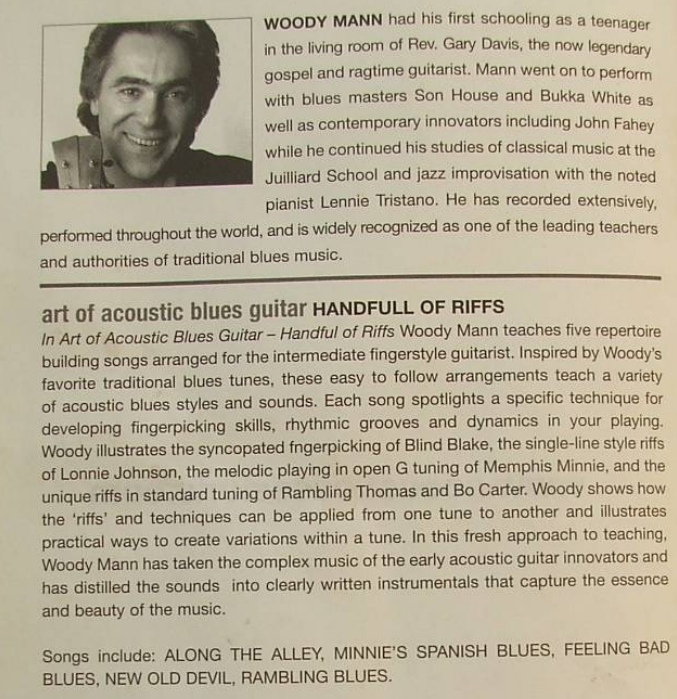
\includegraphics[width=17cm,height=17.552cm]{lebluessupportsmethodes-img49.png}
\end{center}




\clearpage\section[Beginning blus guitar rhythm and solos with Al
Ek]{Beginning blus guitar rhythm and solos with Al Ek}
\hypertarget{RefHeadingToc114973218262}{}\ \ 1. M\'ethode avec Groove
(shuffle, rock{\textquotesingle}n roll, mojo, slow blues, boogaloo,
backwards

\ \ \ \ \ \ \ \ \ \ \ shuffle




\begin{center}
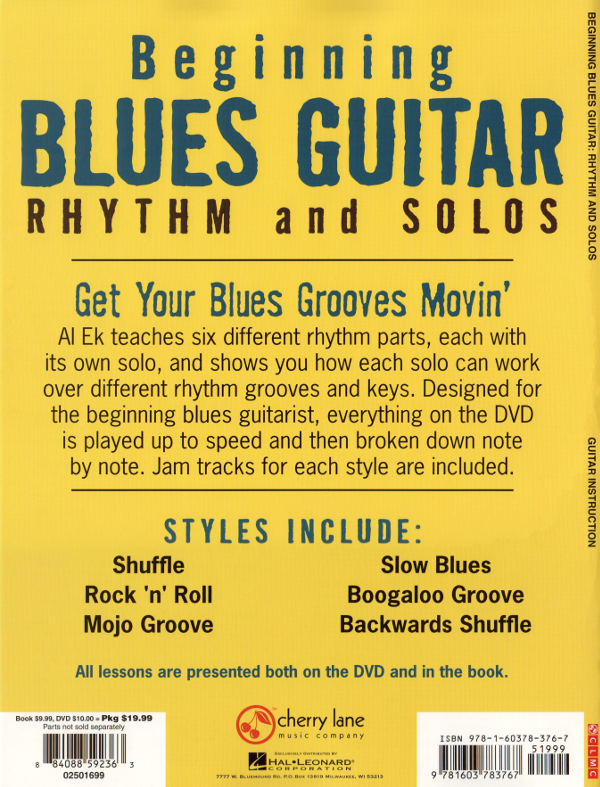
\includegraphics[width=17cm,height=22.306cm]{lebluessupportsmethodes-img50.jpg}
\end{center}
\clearpage

\begin{center}
\includegraphics[width=17cm,height=6.292cm]{lebluessupportsmethodes-img51.jpg}
\end{center}



\clearpage


\section[Beginning blues lead guitar with steve trovato]{Beginning
blues lead guitar with steve trovato}
\hypertarget{RefHeadingToc116973218262}{}




\begin{center}
\includegraphics[width=12.488cm,height=24.012cm]{lebluessupportsmethodes-img52.png}
\end{center}





\begin{center}
\includegraphics[width=16.768cm,height=22.052cm]{lebluessupportsmethodes-img53.png}
\end{center}




\clearpage\section[Beginning blues rhythm guitar with steve
trovato]{Beginning blues rhythm guitar with steve trovato}
\hypertarget{RefHeadingToc118973218262}{}

\begin{center}
\includegraphics[width=12.52cm,height=22.555cm]{lebluessupportsmethodes-img54.png}
\end{center}






\clearpage

\begin{center}
\includegraphics[width=15.954cm,height=19.419cm]{lebluessupportsmethodes-img55.png}
\end{center}





\section[Berklee workshop jazz guitar techniques modal
voicings]{Berklee workshop jazz guitar techniques modal voicings}
\hypertarget{RefHeadingToc120973218262}{}Du jazz tr\`es \'evolu\'e.
Int\'eressant mais pas encore pour moi.






\begin{center}
\includegraphics[width=10.291cm,height=14.469cm]{lebluessupportsmethodes-img56.png}
\end{center}
\clearpage


\section[Beyond Basics Acoustic Slide Guitar with Keith Wyatt]{Beyond
Basics Acoustic Slide Guitar with Keith Wyatt}
\hypertarget{RefHeadingToc122973218262}{}1. Du slide pas mal du tout.






\begin{center}
\includegraphics[width=6.348cm,height=7.089cm]{lebluessupportsmethodes-img57.png}
\end{center}



\clearpage


\section[Beyond basics solo acoustic blues guitar with keith
Wyatt]{Beyond basics solo acoustic blues guitar with keith Wyatt}
\hypertarget{RefHeadingToc124973218262}{}


Du blues acoustique. De tr\`es bonnes explications mais pas de table des
mati\`eres. Il faut regarder tout la vid\'eo pour comprendre o\`u il
va.



\begin{center}
\includegraphics[width=7.62cm,height=10.668cm]{lebluessupportsmethodes-img58.jpg}
\end{center}



\clearpage


\section[Blues by the book wikth roy Book Binder]{Blues by the book
wikth roy Book Binder}
\hypertarget{RefHeadingToc126973218262}{}


T\'el\'echargement incomplet et inexploitable.




\clearpage


\section[Bottleneck Slide Guitar with Fred Solokow]{Bottleneck Slide
Guitar with Fred Solokow}
\hypertarget{RefHeadingToc128973218262}{}1. Du slide mais pas convaincu.
A garder sous le coude.





\begin{center}
\includegraphics[width=13.518cm,height=17.037cm]{lebluessupportsmethodes-img59.png}
\end{center}
\clearpage


\section[Contemporary acoustic jazz guitar with Charlie
Byrd]{Contemporary acoustic jazz guitar with Charlie Byrd}
\hypertarget{RefHeadingToc130973218262}{}Du jazz sur guitare acoustique.






\begin{center}
\includegraphics[width=14.444cm,height=19.496cm]{lebluessupportsmethodes-img60.png}
\end{center}
\clearpage


\section[Effortless Guitar {}- Essential Blues Guitar ]{Effortless
Guitar - Essential Blues Guitar }
\hypertarget{RefHeadingToc132973218262}{}1. Guitare \'electrique. Non






\begin{center}
\includegraphics[width=9.393cm,height=13.229cm]{lebluessupportsmethodes-img61.jpg}
\end{center}






\begin{center}
\includegraphics[width=6.137cm,height=5.978cm]{lebluessupportsmethodes-img62.png}
\end{center}
\clearpage


\section[GPA\_04\_chicago\_blues.iso]{GPA\_04\_chicago\_blues.iso}
\hypertarget{RefHeadingToc134973218262}{}\ \  1. Des morceaux
d\'etaill\'es pour la guitare et des backtrack. Sweet home chicago

\ \ \ \ \ \ \ \ \ \ \ \ notamment.

1. All your love (I miss loving)

2. Easy Baby

3. I ain{\textquotesingle}t got you

4. I{\textquotesingle}m your hoochi coochie main

5. Killing floor

6. Mary had a little lamb

7. Messin{\textquotesingle} with the kid

8. Sweet home chicago






\begin{center}
\includegraphics[width=17cm,height=24.276cm]{lebluessupportsmethodes-img63.jpg}
\end{center}



\clearpage

\begin{center}
\includegraphics[width=17cm,height=4.78cm]{lebluessupportsmethodes-img64.jpg}
\end{center}





\begin{center}
\includegraphics[width=17cm,height=4.78cm]{lebluessupportsmethodes-img65.jpg}
\end{center}


\begin{center}
\includegraphics[width=17cm,height=4.78cm]{lebluessupportsmethodes-img66.jpg}
\end{center}






\clearpage\section[GPA\_23\_Blues\_classic]{GPA\_23\_Blues\_classic}
\hypertarget{RefHeadingToc136973218262}{}\ \  1. Boom boom

\ \  2. Cold Shot

\ \  3. Dust my Broom

\ \  4. Frosty

\ \  5. Further on up the road

\ \  6. Paying the cost to be the boss

\ \  7. The sky is crying

8. Steppin{\textquotesingle} out






\begin{center}
\includegraphics[width=13.968cm,height=17.791cm]{lebluessupportsmethodes-img67.jpg}
\end{center}









\clearpage







\begin{center}
\includegraphics[width=17cm,height=4.78cm]{lebluessupportsmethodes-img68.jpg}
\end{center}





\begin{center}
\includegraphics[width=17cm,height=4.78cm]{lebluessupportsmethodes-img69.jpg}
\end{center}


\begin{center}
\includegraphics[width=17cm,height=4.78cm]{lebluessupportsmethodes-img70.jpg}
\end{center}



\clearpage\section[GPA{}-35\_BB\_King]{GPA-35\_BB\_King}
\hypertarget{RefHeadingToc138973218262}{}1. Gambler{\textquotesingle}s
Blues

2. Just like a woan

3. Paying the cost to be the boss

4. Rock me baby

5. Sweet little angel

6. Sweet sixteen

7. the thrill is gone

8. You upset me baby









\begin{center}
\includegraphics[width=13.995cm,height=17.713cm]{lebluessupportsmethodes-img71.jpg}
\end{center}






\clearpage

\begin{center}
\includegraphics[width=17cm,height=11.538cm]{lebluessupportsmethodes-img72.jpg}
\end{center}







\clearpage\section[Guitar Lab 50 Acoustic Blues Guitar Licks You Must
Know]{Guitar Lab 50 Acoustic Blues Guitar Licks You Must Know}
\hypertarget{RefHeadingToc140973218262}{}1. Bien. Blues accoustique.
Fichiers avi + book.






\begin{center}
\includegraphics[width=14.894cm,height=19.313cm]{lebluessupportsmethodes-img73.png}
\end{center}






\clearpage\section[Guitar Lab 50 Blues Guitar Licks You Must
Know]{Guitar Lab 50 Blues Guitar Licks You Must Know}
\hypertarget{RefHeadingToc142973218262}{}1. Bien \'electrique. Des
classiques et des plus modernes. Faire le tri.






\begin{center}
\includegraphics[width=17cm,height=21.652cm]{lebluessupportsmethodes-img74.jpg}
\end{center}



\clearpage

\begin{center}
\includegraphics[width=17cm,height=11.43cm]{lebluessupportsmethodes-img75.jpg}
\end{center}


\begin{center}
\includegraphics[width=17cm,height=4.697cm]{lebluessupportsmethodes-img76.jpg}
\end{center}


\begin{center}
\includegraphics[width=17cm,height=4.715cm]{lebluessupportsmethodes-img77.jpg}
\end{center}









\clearpage\section[Guitar Lab 50 Blues Rock Guitar Licks You Must
Know]{Guitar Lab 50 Blues Rock Guitar Licks You Must Know}
\hypertarget{RefHeadingToc144973218262}{}1. Electrique. Tr\`es blues
rock. Je n{\textquotesingle}ai pas creuse de trop.






\begin{center}
\includegraphics[width=17cm,height=21.652cm]{lebluessupportsmethodes-img78.jpg}
\end{center}


\begin{center}
\includegraphics[width=17cm,height=11.488cm]{lebluessupportsmethodes-img79.jpg}
\end{center}


\begin{center}
\includegraphics[width=17cm,height=4.715cm]{lebluessupportsmethodes-img80.jpg}
\end{center}








\begin{center}
\includegraphics[width=17cm,height=4.715cm]{lebluessupportsmethodes-img81.jpg}
\end{center}









\clearpage


\section[Guitar Lab 50 Blues Rock Rhythms You Must Know]{Guitar Lab
50 Blues Rock Rhythms You Must Know}
\hypertarget{RefHeadingToc146973218262}{}1. Electrique. Tr\`es rock. Pas
mon style.






\begin{center}
\includegraphics[width=17cm,height=15.007cm]{lebluessupportsmethodes-img82.jpg}
\end{center}






\clearpage

\begin{center}
\includegraphics[width=17cm,height=7.479cm]{lebluessupportsmethodes-img83.jpg}
\end{center}


\begin{center}
\includegraphics[width=17cm,height=5.976cm]{lebluessupportsmethodes-img84.jpg}
\end{center}


\begin{center}
\includegraphics[width=17cm,height=5.976cm]{lebluessupportsmethodes-img85.jpg}
\end{center}






\clearpage


\section[Guitar Lab 50 Eclectic Blues Guitar Licks You Must
Know]{Guitar Lab 50 Eclectic Blues Guitar Licks You Must Know}
\hypertarget{RefHeadingToc148973218262}{}1. Electrique. Blues moderne.
Peut-\^etre \`a creuser quelques rythmes.






\begin{center}
\includegraphics[width=17cm,height=25.904cm]{lebluessupportsmethodes-img86.jpg}
\end{center}


\begin{center}
\includegraphics[width=17cm,height=6.639cm]{lebluessupportsmethodes-img87.jpg}
\end{center}


\begin{center}
\includegraphics[width=17cm,height=12.084cm]{lebluessupportsmethodes-img88.png}
\end{center}








\clearpage\section[Guitar Lab 50 jazz Guitar Licks You Must
Know]{Guitar Lab 50 jazz Guitar Licks You Must Know}
\hypertarget{RefHeadingToc150973218262}{}Pas creus\'e.



\begin{center}
\includegraphics[width=17cm,height=21.652cm]{lebluessupportsmethodes-img89.jpg}
\end{center}



\clearpage

\begin{center}
\includegraphics[width=17cm,height=11.435cm]{lebluessupportsmethodes-img90.jpg}
\end{center}


\begin{center}
\includegraphics[width=17cm,height=4.731cm]{lebluessupportsmethodes-img91.jpg}
\end{center}


\begin{center}
\includegraphics[width=17cm,height=4.747cm]{lebluessupportsmethodes-img92.jpg}
\end{center}



\clearpage


\section[Guitar Lab 50 Texas Blues Guitar Licks You Must Know]{Guitar
Lab 50 Texas Blues Guitar Licks You Must Know}
\hypertarget{RefHeadingToc152973218262}{}1. Electrique. Bien, voire
m\^eme tr\`es bien.






\begin{center}
\includegraphics[width=17cm,height=14.974cm]{lebluessupportsmethodes-img93.jpg}
\end{center}












\clearpage

\begin{center}
\includegraphics[width=17cm,height=7.479cm]{lebluessupportsmethodes-img94.jpg}
\end{center}


\begin{center}
\includegraphics[width=17cm,height=5.976cm]{lebluessupportsmethodes-img95.jpg}
\end{center}


\begin{center}
\includegraphics[width=17cm,height=5.976cm]{lebluessupportsmethodes-img96.jpg}
\end{center}
\clearpage


\section[Guitar Legendary Licks Blues Masters by the Bar with Dave
Celentano]{Guitar Legendary Licks Blues Masters by the Bar with Dave
Celentano}
\hypertarget{RefHeadingToc154973218262}{}1. A creuser, des trucs bien
comme la premi\`ere lick.






\begin{center}
\includegraphics[width=12.277cm,height=12.277cm]{lebluessupportsmethodes-img97.jpg}
\end{center}







\clearpage


\section[Guitar World How to Play Blues and Blues Rock Guitar]{Guitar
World How to Play Blues and Blues Rock Guitar}
\hypertarget{RefHeadingToc156973218262}{}1. Electrique. Des exemples \`a
creuser plus tard.

2. Electrique. Pas mal du tout. D\'emarre \`a la base.






\begin{center}
\includegraphics[width=13.042cm,height=15.212cm]{lebluessupportsmethodes-img98.png}
\end{center}






\clearpage

\begin{center}
\includegraphics[width=11.957cm,height=16.455cm]{lebluessupportsmethodes-img99.png}
\end{center}









\clearpage

\begin{center}
\includegraphics[width=12.804cm,height=14.312cm]{lebluessupportsmethodes-img100.png}
\end{center}
\clearpage


\section[How To Play Fingerstyle Blues Guitar Solos with Mark
Hanson]{How To Play Fingerstyle Blues Guitar Solos with Mark Hanson}
\hypertarget{RefHeadingToc158973218262}{}1. Accoustique picking \`a la
Soig Sib\'eril. Non






\begin{center}
\includegraphics[width=12.929cm,height=18.122cm]{lebluessupportsmethodes-img101.jpg}
\end{center}







\clearpage

\begin{center}
\includegraphics[width=16.903cm,height=12.778cm]{lebluessupportsmethodes-img102.png}
\end{center}
\clearpage


\section[Improvisation (Initiation \`a
l{\textquotesingle})]{Improvisation (Initiation \`a
l{\textquotesingle})}
\hypertarget{RefHeadingToc160973218262}{}1. Excellent. A pratiquer.
Tr\`es bien expliqu\'e pour d\'ebuter.






\begin{center}
\includegraphics[width=17cm,height=14.533cm]{lebluessupportsmethodes-img103.png}
\end{center}






\clearpage

\begin{center}
\includegraphics[width=17cm,height=9.246cm]{lebluessupportsmethodes-img104.png}
\end{center}



\clearpage


\section[Improvisation avec les gammes]{Improvisation avec les
gammes}
\hypertarget{RefHeadingToc162973218262}{}Du travail plus pointu pour
plus tard.



\begin{center}
\includegraphics[width=17cm,height=9.841cm]{lebluessupportsmethodes-img105.png}
\end{center}


\begin{center}
\includegraphics[width=17cm,height=11.767cm]{lebluessupportsmethodes-img106.png}
\end{center}
\clearpage

\begin{center}
\includegraphics[width=17cm,height=11.555cm]{lebluessupportsmethodes-img107.png}
\end{center}


\begin{center}
\includegraphics[width=17cm,height=12.771cm]{lebluessupportsmethodes-img108.png}
\end{center}
\clearpage\section[Jazz for the electric blues guitarist with Adrian
Ingram]{Jazz for the electric blues guitarist with Adrian Ingram}
\hypertarget{RefHeadingToc164973218262}{}Pas creus\'e car jazz.



\begin{center}
\includegraphics[width=11.716cm,height=8.869cm]{lebluessupportsmethodes-img109.png}
\end{center}



\begin{center}
\includegraphics[width=14.76cm,height=15.503cm]{lebluessupportsmethodes-img110.png}
\end{center}
\clearpage\section[Jazz guitar mastery with John Stowell]{Jazz guitar
mastery with John Stowell}
\hypertarget{RefHeadingToc166973218262}{}Du pur jazz. Mis de c\^ot\'e
pour l{\textquoteright}instant.



\begin{center}
\includegraphics[width=8.398cm,height=11.188cm]{lebluessupportsmethodes-img111.jpg}
\end{center}



\clearpage

\begin{center}
\includegraphics[width=13.704cm,height=19.232cm]{lebluessupportsmethodes-img112.png}
\end{center}






\clearpage\section[Keith Wyatt {}- Blues Guitar Basics (Book +
Cd)/Audio]{Keith Wyatt - Blues Guitar Basics (Book + Cd)/Audio}
\hypertarget{RefHeadingToc168973218262}{}\ \  1. Electrique. Explication
de Keith Wyatt bien.

\ \  2. Excellent. Electrique. Des \'el\'ements pr\'ecis et bien
d\'etaill\'es en mp3 seulement. Pas

\ \ \ \ \ \ \ \ \ \ \ \ de morceaux par contre, que des points pr\'ecis.



\begin{center}
\includegraphics[width=13.757cm,height=17.829cm]{lebluessupportsmethodes-img113.png}
\end{center}









\clearpage

\begin{center}
\includegraphics[width=17cm,height=16.953cm]{lebluessupportsmethodes-img114.png}
\end{center}





\clearpage\section[Le Blues acoustique Alain Giroux French Ebook
PDF/CD]{Le Blues acoustique Alain Giroux French Ebook PDF/CD}
\hypertarget{RefHeadingToc170973218262}{}\ \  1. De tr\`es bons exemples
de blues accoustique.

\ \  \ \ \ 1. Lightnin{\textquotesingle} hopkins, Lonnie Jonhson,
Scraper Blackwell, Robert Johnson, basses en

\ \ \ \ \ \ \ \ \ \ \ \ \ \ \ slap \`a la John Lee Hooker, Big Joe
Williams etc., style Mississipi (binaire)

\ \ \ \ \ \ \ \ \ \ \ \ \ \ \ open tuning de D et G,
\ (j{\textquotesingle}aime)









\begin{center}
\includegraphics[width=17cm,height=23.451cm]{lebluessupportsmethodes-img115.jpg}
\end{center}









\clearpage

\begin{center}
\includegraphics[width=14.469cm,height=17.247cm]{lebluessupportsmethodes-img116.png}
\end{center}





\clearpage


\section[Learn American Blues in 6 Weeks]{Learn American Blues in 6
Weeks}
\hypertarget{RefHeadingToc172973218262}{}1. Electrique. Guitare lead.
Tr\`es bien. Du basique. Lick Library



\begin{center}
\includegraphics[width=8.996cm,height=13.044cm]{lebluessupportsmethodes-img117.jpg}
\end{center}





\begin{center}
\includegraphics[width=8.729cm,height=7.671cm]{lebluessupportsmethodes-img118.png}
\end{center}






\clearpage

\begin{center}
\includegraphics[width=7.883cm,height=8.2cm]{lebluessupportsmethodes-img119.png}
\end{center}





\begin{center}
\includegraphics[width=8.729cm,height=7.671cm]{lebluessupportsmethodes-img120.png}
\end{center}




\begin{center}
\includegraphics[width=8.703cm,height=8.121cm]{lebluessupportsmethodes-img121.png}
\end{center}




\clearpage

\begin{center}
\includegraphics[width=10.026cm,height=9.047cm]{lebluessupportsmethodes-img122.png}
\end{center}





\begin{center}
\includegraphics[width=8.147cm,height=8.068cm]{lebluessupportsmethodes-img123.png}
\end{center}



\clearpage


\section[Learn And Master Blues Guitar]{Learn And Master Blues
Guitar}
\hypertarget{RefHeadingToc174973218262}{}
Electrique. Super excellent car explications qui utilisent les musiciens du groupe. Lead et rythm.
Parmi les supports vidéos les workshop ont l'air moins complets que les sessions. A vérifier.
\subsection{Session One. Les Bases du Blues : forme, accord 7, riffs à partir des accords.}
	\begin{itemize}
	\item \textbf{Objectifs}
		\begin{itemize}
		\item Apprendre la forme du 12-bar blues.
		\item Apprendre les formes ouvertes communes et d\'eplaçables des accords 7.
		\item Apprendre à reconnaître les degr\'es I IV et V.
		\item Improviser des riffs bas\'e sur les empreintes d'accords.
		\end{itemize}
	\end{itemize}	
	
	
	\begin{itemize}
	\item \textbf{Idées clefs}
		\begin{itemize}
		\item Le blues est une progression en 12 mesures
		\item Les blues utilise 3 accords principaux, le I, le IV et le V dans n'importe quelle clef.
		\item Ecoutez la note de basse de l'accord pour vous aider à d\'eterminer de quel degr\'e il s'agit.
		\item Quand vous apprenez un nouveau riff :
		
			\begin{itemize}
			\item Apprenez le riff avec un doigt\'e propre et pr\'ecis.
			\item D\'eplacez le à diff\'erents endroit du manche.
			\item Exp\'erimentez diff\'erentes variations.
			\end{itemize}
			
		\item La progression blues à beaucoup de variations.
		\item Une variation courante est d'ins\'erer l'accord IV à la deuxième mesure.
		\item A la répétition de la forme, mettre un accord V dans la dernière mesure.
		\item Une autre variation commune est de mettre un accord IIm mesure 9 qui va aller sur l'accord V mesure 10.
		\end{itemize}
		
	\end{itemize}
	
	
	\begin{itemize}
	\item \textbf{Termes}
	\begin{itemize}
		\item Accords 7. Construits avec 1 3 5 $\flat$7 dans n'importe quelle clef.
		\item Accords ouverts (open chords) : formes d'accords de guitare qui utilisent des cordes à vide.
		\item Accords mobiles (moveable chords) : formes d'accords de guitare qui n'utilisent pas de cordes à vides et sont de ce fait déplaçables à différents endroits du manche.
		\item Accords barrés : accords qui utilisent un doigt pour couvrir plus d'une corde dans la forme de l'accord.
		\end{itemize}
	\end{itemize}

	\begin{itemize}
	\item \textbf{Choses à faire}
		\begin{itemize}
		\item Jouer et m\'emoriser tous les open chords et moveable accords 7.
		\item M\'emoriser les notes sur les cordes 5 et 6 de la guitare.
		\end{itemize}
	\end{itemize}
	
	\begin{itemize}
	\item \textbf{Suggestions d'écoute}
		\begin{itemize}
		\item B.B. King : \emph{Live from the Cook County Jail}
		\item Muddy Waters : \emph{The Complete Plantation Recordings}
		\item Robert Cray : \emph{Live from Across the Pond}
		\item Eric Clapton : \emph{Me and Mr. Johnson}
		\item Robert Jonhson : \emph{The Complete Recording : Robert Jonhson}
		\end{itemize}
	\end{itemize}

	


	\begin{itemize}
	\item \textbf{Devoirs pour cette session.}
		\begin{itemize}
		\item[Mémoriser la 12-bar blues chord progression.]
		\item[Jouer la progression en A, C, D, E et G.]
		\item[Apprendre tous les open and moveable 7t chords étudiés.]
		\item[Expérimenter des blues-riffs à partir des accords 7 barrés.]
		\end{itemize}
	\end{itemize}


\subsection{Session Two. Les incontournables : blues note, bends, boggie-woogie en 5tes.}
\subsubsection{Objectifs}
\begin{itemize}
\item Apprendre les blues notes et comprendre comment les utiliser.
\item Entendre les blues notes.
\item Jouer les bends efficacement.
\item Apprendre les motifs de boogie-woogie en 5th.
\end{itemize}
\subsubsection{Idées clefs}
\begin{itemize}
\item Les blues notes sont $\flat$3, $\flat$5 et $\flat$7
\item $\flat$3 et 3 peuvent se substituer l'une à l'autre, selon le son que vous voulez entendre.
\item Quand vous jouez du blues, ne JAMAIS utiliser 7, TOUJOURS utiliser $\flat$7.
\item Utilisez $\flat$5 autant que vous voulez, soyez simplement certain de la résoudre sur 4 ou 5.
\item La capacité de se rappeler sans hésitations 3, 5 et 7 dans n'importe quelle clef est une des compétences les plus importantes que vous apprendrez. Pratiquer les de mémoire tous les jours.
\item Ecoutez et soyez capable de reconnaître les blues notes à l'oreille.
\item quand vous faites un bend, viser une note précise.
\item Faire un bend requiert de la force et du contrôle de la main.
\item D'abord pratiquez les bend sur des cordes à faibles tirant. Après ce premier apprentissage changez les cordes pour des cordes à plus fort tirant. Quand votre main à acquis en force et précision remettez des cordes à faibles tirant.
\item Quand vous pratiquez des bends :
\begin{itemize}
\item Utilisez les autres doigts pour aider et pousser sur la corde.
\item Poser le pouce légèrement derrière le manche comme point de support.
\item Les bends demandent de la force de la part de la main. Cette force prend du temps à se développer. Ne vous découragez pas si vos bends ne sonnent pas correctement au début. Ayez une pratique journalière pour donner le temps aux muscles de vos mains de se développer.
\item Quand vous apprenez une lick, jouez là à tous les endroits du manche et à toutes les octaves. Apprenez la lick, puis expérimentez des variations mélodiques sur le même shéma de doigts.
\end{itemize}
\subsubsection{Devoirs}
\begin{itemize}
\item Mémorisez les blues notes.
\item Comprenez le rôle de chacune des blues note.
\item Pratiquez les bends avec une technique parfaite.
\item Pratiquez chaque jours les trois types de bends, demi-ton, ton, ton et demi.
\end{itemize}
\end{itemize}

\subsection{Session Three. Gammes blues, technique de picking, faire le meilleur à partir d'idées simple.}
\subsubsection{Objectifs}
\begin{itemize}
\item Comprendre les différentes gammes utilisées en blues.
\item Jouer en utilisant le picking avec force.
\item Apprendre l'accord Sus dans les riffs blues avec le hammer-on.
\end{itemize}
\subsubsection{Idées clefs}
\begin{itemize}
\item La gamme majeure est une combinaison de demi-tons et de tons construite à partir d'une tonique. 
\end{itemize}

\subsubsection{Termes}
\begin{itemize}
\item Un demi-ton est l'intervalle entre une note et la note suivante distante d'une frette sur la guitare.
\item Un ton est l'intervalle de 2 demi-tons, ce qui équivaut à une distance de 2 frettes sur la guitare.
\item Une position est une rangée de cases sur le manche de la guitare définie par la case sur laquelle est posée l'index.
\item Comprendre les gammes majeures et les tonalités, connaître quelles sont les notes des accords est un grand bénéfice pour jouer des solos.
\item Jouez toutes les gammes chaque jour pendant deux semaines et vous aurez les schémas dans la mémoire gestuelle, prêts à servir en jeu réel ou en situation de solo.
\item Une gamme facile à utiliser en blues est la pentatonique mineure. Par exemple, dans un blues en A, vous pouvez utiliser la gamme de La mineur pentatonique.
\item Ajoutez la blues note à la pentatonique mineure pour un son encore plus bluesy.
\item Beaucoup de joueurs jouent trop soft. N'ayez pas peur de jouer et pincer avec force, spécialement quand vous jouez du blues.
\item Exercice d'entraînement au solo :
\begin{itemize}
\item Solo utilisant seulement 1 note : la tonique.
\item Solo utilisant seulement 1 note : la tonique à différentes octaves.
\item Solo utilisant 1 note : bends et slides sur la tonique à différentes octaves.
\item Solo utilisant seulement 2 notes : des toniques et des sixtes dans toutes les octaves.
\item Solo utilisant 3 notes : 1, 2, $\flat$3 à toutes les octaves.
\item Solo utilisant le même schéma de doigts sur des cordes adjacentes.
\item Toutes les licks jouées sur deux cordes adjacentes peuvent être jouées en utilisant le même schéma de doigts. La seule exception sont les licks jouées sur les cordes 3 et 2.
\item Pratique : travailler une lick que vous aimez, et ensuite jouez la sur toutes les cordes et avec toutes les combinaisons de doigts que vous trouverez.
\end{itemize}
\end{itemize}
\subsubsection{Devoirs}
\begin{itemize}
\item Apprenez les tonalités et leur armure.
\item Jouer les gammes majeures et les exercices de mémoire.
\item Apprenez la forme de la gamme mineure pentatonique, et la forme avec la blue note ajoutée.
\item Pratiquez le bending correct sur les notes sur la gamme mineure pentatonique.
\item Pratiquer le picking avec force.
\item Pratiquer les licks d'oreille et jouez les dans différentes tonalités.
\item Apprenez l'accord Sus dans les schémas blues de hammer-on.
\end{itemize}

\subsection{Session Four. More Blues Tools : accords blues avancés, vibrato, sliding 6ths riff.}


\subsubsection{Objectif}
\begin{itemize}
\item Apprendre les formes d'accords 9èmes, 13èmes et demi-diminués.
\item Comprendre la substitution de l'accord demi-diminué.
\item Entendre la différence entre M6 et $\flat$7.
\item Jouez les riffs mobiles sur la corde 6.
\end{itemize}

\subsubsection{Idées clefs}
\begin{itemize}
\item Notation des accords X7 et XM7, X9 et XM9.
\item Vous pouvez substituer un accord 9 à n'importe quel accord 7.
\item Un accord X9 peut être substitué par un accord demi-diminué construit sur la tierce de cet accord (et inversement).
\item En blues, l'accord 7($\sharp$9) est utilisé comme un substitut de V dans une tonalité.
\item Les accords 13 sont courants en blues.
\item On peut omettre la 5te et la tonique dans les accords complexes.
\item Choisissez des formes d'accords localisées dans la même partie du manche pour éviter de grands sauts.
\item Les accords qui comportent des notes communes font des progressions d'accords cohérentes, qui sonnent.
\item Chaque fois que vous voyez un accord X7 vous pouvez substituer un X9 ou X13.
\item Une légère touche de vibrato donne déjà beaucoup de caractère à votre son.
\item Une idée mélodique simple peut être jouée à différents endroits du manche en utilisant les mêmes doigtés.
\end{itemize}

\subsubsection{Devoirs}
\begin{itemize}
\item Apprendre les accords 9 13 et 7($\sharp$9)
\item Comprendre la subsitution X9 X demi-diminué.
\item Pratiquer avec une bonne position de main et une technique de vibrato propre.
\item Pratiquer et entendre la différence entre 6 et b7 dans les improvisations.
\item Apprendre les schémas mobiles sur les cordes 5 et 6.
\item Apprendre les deux versions de sliding 6ths riff.
\end{itemize}


\subsection{Session Five. La folie des intervalles : intervalles en blues, choisir la note juste, schémas de doigts classiques en blues.}

\subsubsection{Objectifs}
\begin{itemize}
\item Jouez des 3ces, 4tes, 5tes, 6tes sur la guitare.
\item Apprenez quelques expressions blues standards.
\item Jouez les riffs d'intervalles étudiés.
\end{itemize}

\subsubsection{Idées Clefs}
\begin{itemize}
\item Les intervalles couramment utilisés en blues sont 3ces, 4tes, 5tes et 6tes.
\item 4tes et 5tes ont un son très "ouvert".
\item Travaillez le doigté en 3ces de ces riffs dans d'autres clefs qui n'incluent pas de cordes ouvertes. Ce riff est joué souvent sur tout le manche.
\item Toujours pratiquer les nouvelles idées dans des situations musicales réelles. C'est le secret pour les intérioriser. Si vous ne pratiquez pas vos idées dans des situations réelles elles n'auront aucune utilité pour vous.
\end{itemize}

\subsubsection{Devoirs}
\begin{itemize}
\item Pratiquer les intervalles de cette session.
\item Pratiquer les trois formes techniques d'expression.
\item Pratiquer les 4 règles pour choisir les bonnes notes.
\item Apprenez les deux blues finger patterns.
\end{itemize}




\subsection{Section Six. Maîtriser le Blues : types de blues, jouer ce que vous entendez, jouer avec un groupe.}
\subsubsection{Objectifs}
\begin{itemize}
\item Devenir familier avec différents types de blues.
\item Apprendre à donner une touche jazz à une progression d'accords.
\item Jouer des solos à l'oreille.
\item Apprendre les techniques de pull-off et de up-stroke.
\end{itemize}

\subsection{Idées clefs}
\begin{itemize}
\item Le \emph{shuffle} à un feeling sous-jacent en triolet.
\item le feeling du 12/8 est tellement lent que les triolets de croches sont ressentis comme 3 croches pour chacun des 4 temps dans chacune des mesures.
\item Un blues lent en 12/8 est un bon feeling pour pratiquer le solo car il est tellement lent qu'il donne beaucoup de temps au musicien pour penser et expérimenter des idées.
\item Le feeling boogie-woogie est plus rapide, à la \emph{Chuck Berry} ou \emph{The Stray Cats}.  
\item Donner une couleur jazz en ajoutant des notes de couleurs comme des 9èmes, des 13èmes ou des 9$\sharp$.
\item Vous pouvez introduire chaque accord par un accord V7 de sa tonalité, et faire précéder ce dernier d'un IIm.
\item Toutes les techniques utilisées pour donner une couleur jazz aux progressions d'accords peuvent aussi être utilisées dans les solos. Vous pouvez par exemple jouer un arpège de Cm7 et F7 avant d'arriver sur un accord de B$\flat$. Vous pouvez faire une emphase sur la 9ème ou 13ème (notes de couleur), sur un accord de votre solo même si l'accord écrit est un simple X7. Vous pouvez jouer un passage chromatique qui va vous amener sur l'accord désiré.
\item Cherchez les opportunités de jouer avec un groupe. Rien ne peut mieux inspirer votre créativité que de jouer régulièrement en groupe. Jouer avec un groupe est l'un des moyens les plus rapides pour improviser sur votre instrument. Si vous voulez accélérer votre apprentissage, allez au delà de vos peurs et cherchez un groupe de musiciens.
\item Utiliser les jam-along, play-along, backtracks, pour vous aider à apprendre à improviser. Pratiquer avec des enregistrements offre la pratique nécéssaire pour jouer ce que l'on entend en solo.
\end{itemize}

\subsubsection{Devoirs}
\begin{itemize}
\item Devenir familier des différents styles de blues.
\item Jouer avec les différents enregistrements des jam-alongs.
\item Pratiquer le solo en utilisant l'oreille comme guide.
\item Pratiquer les techniques de upstroke et de pull-off.
\end{itemize}

\subsubsection{Très important}
La capacité à trouver sans hésitations les 3ces, 5tes et 7èmes dans n'importe quelle tonalité est l'une des choses les plus importantes que vous devez apprendre. Dites-les de mémoire chaque jour.




\begin{center}
\includegraphics[width=17cm,height=13.765cm]{lebluessupportsmethodes-img124.png}
\end{center}












\clearpage




\begin{center}
\includegraphics[width=17cm,height=16.628cm]{lebluessupportsmethodes-img125.png}
\end{center}





\clearpage\section[Learn Electric Blues Guitar in 6 Weeks]{Learn
Electric Blues Guitar in 6 Weeks}
\hypertarget{RefHeadingToc176973218262}{}1. Bien du basique comme /Learn
American Blues in 6 Weeks/ \ . Lick Library






\begin{center}
\includegraphics[width=9.366cm,height=12.039cm]{lebluessupportsmethodes-img126.jpg}
\end{center}




\clearpage\section[Learn Slide Guitar]{Learn Slide Guitar}
\hypertarget{RefHeadingToc178973218262}{}1. Electrique. De la slide bien
agressive. Pas mal.






\begin{center}
\includegraphics[width=11.906cm,height=8.652cm]{lebluessupportsmethodes-img127.jpg}
\end{center}




\begin{center}
\includegraphics[width=17cm,height=11.333cm]{lebluessupportsmethodes-img128.jpg}
\end{center}





\begin{center}
\includegraphics[width=17cm,height=11.333cm]{lebluessupportsmethodes-img129.jpg}
\end{center}
\begin{center}
\includegraphics[width=17cm,height=11.333cm]{lebluessupportsmethodes-img130.jpg}
\end{center}






\section[Learn to Play Blues Lead Guitar]{Learn to Play Blues Lead
Guitar}
\hypertarget{RefHeadingToc180973218262}{}1. Electrique. Bien dans la
veine de Lick Library






\begin{center}
\includegraphics[width=9.208cm,height=13.229cm]{lebluessupportsmethodes-img131.jpg}
\end{center}





\begin{center}
\includegraphics[width=12.196cm,height=6.719cm]{lebluessupportsmethodes-img132.png}
\end{center}





\clearpage


\section[Learn to Play Your Own Blues Solos]{Learn to Play Your Own
Blues Solos}
\hypertarget{RefHeadingToc182973218262}{}1. Lick Library.






\begin{center}
\includegraphics[width=9.155cm,height=13.229cm]{lebluessupportsmethodes-img133.jpg}
\end{center}





\begin{center}
\includegraphics[width=12.01cm,height=6.824cm]{lebluessupportsmethodes-img134.png}
\end{center}



\clearpage


\section[Learn to Play Your Own Jazz Solos]{Learn to Play Your Own
Jazz Solos}
\hypertarget{RefHeadingToc184973218262}{}1. Jazz electrique. Library
Lick






\begin{center}
\includegraphics[width=12.143cm,height=5.449cm]{lebluessupportsmethodes-img135.png}
\end{center}





\clearpage\section[Quick Licks {}- Jeff Beck {}- Slow Blues]{Quick
Licks - Jeff Beck - Slow Blues}
\hypertarget{RefHeadingToc186973218262}{}T\'el\'echargement incomplet et
inexploitable.


\clearpage\section[Real Blues Guitar with Keny Chipkin]{Real Blues
Guitar with Keny Chipkin}
\hypertarget{RefHeadingToc188973218262}{}1. De bons exemples et un livre
en pdf. Le son semble d\'ecal\'e sur la fin de la vid\'eo.






\begin{center}
\includegraphics[width=10.001cm,height=13.229cm]{lebluessupportsmethodes-img136.jpg}
\end{center}




\clearpage

\begin{center}
\includegraphics[width=11.906cm,height=15.584cm]{lebluessupportsmethodes-img137.jpg}
\end{center}



\clearpage




\begin{center}
\includegraphics[width=16.374cm,height=17.644cm]{lebluessupportsmethodes-img138.png}
\end{center}
\clearpage\section[The Art of Blues Rhythm with Robben Ford]{The Art
of Blues Rhythm with Robben Ford}
\hypertarget{RefHeadingToc190973218262}{}1. Tr\`es bien. Uniquement du
rythme jusqu{\textquotesingle}\`a des choses funky.






\begin{center}
\includegraphics[width=13.106cm,height=18.052cm]{lebluessupportsmethodes-img139.jpg}
\end{center}







\clearpage

\begin{center}
\includegraphics[width=13.005cm,height=18.034cm]{lebluessupportsmethodes-img140.jpg}
\end{center}



\clearpage

\begin{center}
\includegraphics[width=16.702cm,height=19.385cm]{lebluessupportsmethodes-img141.png}
\end{center}





\clearpage\section[The Legendary Blues Guitar of Josh White]{The
Legendary Blues Guitar of Josh White}
\hypertarget{RefHeadingToc398973218262}{}1. Guitare
d{\textquotesingle}accompagnement du chant. Pas pour moi.



\begin{center}
\includegraphics[width=14.446cm,height=20.373cm]{lebluessupportsmethodes-img142.jpg}
\end{center}





\clearpage\section[Ultimate guitar techniques {}- Scale
Shapes.]{Ultimate guitar techniques - Scale Shapes.}
\hypertarget{RefHeadingToc194973218262}{}T\'el\'echargement incomplet et
inexploitable.

\clearpage\section{Vidéos}
\subsubsection{B.B.King Clinic}
A voir absolument pour tous les guitaristes.


\clearpage

\chapter[Basse et Contrebasse]{Basse et Contrebasse}
\hypertarget{RefHeadingToc277322781263}{}

\section{Progressive Bass Blues.pdf}

Très bien pour débuter, rempli très bien son rôle.
Des exemples de débuts, fin, Stop Time Blues, lead-in. Termine avec quelques techniques avancées, hammer-on, pull-off, harmoniques, slap, popping, gosht notes.

\begin{center}
\includegraphics[width=11.481cm,height=15.82cm]{lebluessupportsmethodes-img143.png}
\end{center}




\begin{center}
\includegraphics[width=12.196cm,height=18.44cm]{lebluessupportsmethodes-img144.png}
\end{center}
\clearpage\section{Bass Lines - Bob Cranshaw}
Blues façon jazz. Du Aebeersold. Pas le style qu'on veut faire avec Xavier.

\begin{center}
\includegraphics[width=15.051cm,height=19.523cm]{lebluessupportsmethodes-img145.png}
\end{center}


\begin{center}
\includegraphics[width=17cm,height=17.699cm]{lebluessupportsmethodes-img146.png}
\end{center}
\clearpage\section{The improviser{\textquotesingle}s bass method}



\begin{center}
\includegraphics[width=13.862cm,height=18.493cm]{lebluessupportsmethodes-img147.png}
\end{center}





\begin{center}
\includegraphics[width=13.28cm,height=18.043cm]{lebluessupportsmethodes-img148.png}
\end{center}


\begin{center}
\includegraphics[width=12.831cm,height=18.517cm]{lebluessupportsmethodes-img149.png}
\end{center}
\clearpage\section[Bass{}-Play{}-Along{}-Blues.pdf]{Bass-Play-Along-Blues.pdf}


\begin{center}
\includegraphics[width=12.513cm,hesight=17.089cm]{lebluessupportsmethodes-img150.png}
\end{center}


\clearpage\section{Ed Friedland - Blues Bass -- 2005}
Très très très bien. Nous fait pénétrer au coeur de la culture des musiciens de blues sur tous les trucs de groupes. Des explications claires.


\begin{center}
\includegraphics[width=12.169cm,height=16.718cm]{lebluessupportsmethodes-img151.png}
\end{center}





\begin{center}
\includegraphics[width=16.191cm,height=18.597cm]{lebluessupportsmethodes-img152.png}
\end{center}
\clearpage\section{Expanding Walking Bass Lines - Ed Friedland}
Second volet d{\textquoteright}un prof r\'eput\'e aux States.



\begin{center}
\includegraphics[width=11.693cm,height=16.111cm]{lebluessupportsmethodes-img158.png}
\end{center}





\begin{center}
\includegraphics[width=15.714cm,height=20.052cm]{lebluessupportsmethodes-img159.png}
\end{center}


\begin{center}
\includegraphics[width=15.395cm,height=8.174cm]{lebluessupportsmethodes-img160.png}
\end{center}



\clearpage
\section{Mel Bay{\textquotesingle}s Famous Blues Bass Lines
- by Larry McCabe}

Un réservoir de pattern. Quelques explications bien utiles au début. A garder en réserver pour arranger ou proposer des exemples aux élèves.

\begin{center}
\includegraphics[width=17cm,height=11.823cm]{lebluessupportsmethodes-img153.png}
\end{center}
\clearpage


\section{Bass Tab White Pages - Hal Leonard}
Des partitions de basses pour des morceaux blues, rock etc.



\begin{center}
\includegraphics[width=14.286cm,height=20.025cm]{lebluessupportsmethodes-img154.png}
\end{center}


\begin{center}
\includegraphics[width=14.259cm,height=19.893cm]{lebluessupportsmethodes-img155.png}
\end{center}









\clearpage\section{Mulot, Pascal - La Technique du Slap a la Basse}
Quelques exercices fondamentaux pour le slap.



\begin{center}
\includegraphics[width=17cm,height=13.4cm]{lebluessupportsmethodes-img156.png}
\end{center}
\clearpage\section{Methode Basse - Bass Aerobics}
Tout est dans le titre. Une ann\'ee d{\textquoteright}exercices de
gymnastique pour bassiste.



\begin{center}
\includegraphics[width=17cm,height=14.198cm]{lebluessupportsmethodes-img157.png}
\end{center}

\clearpage\section{Jaco Pastorius - Bass Signature Licks}


\begin{center}
\includegraphics[width=14.841cm,height=19.734cm]{lebluessupportsmethodes-img161.png}
\end{center}


\begin{center}
\includegraphics[width=14.76cm,height=19.022cm]{lebluessupportsmethodes-img162.png}
\end{center}
\clearpage\section{Jaco Pastorius - The Greatest Jazz-Fusion Bass
Player}


\begin{center}
\includegraphics[width=12.328cm,height=17.117cm]{lebluessupportsmethodes-img163.png}
\end{center}





\begin{center}
\includegraphics[width=17cm,height=16.323cm]{lebluessupportsmethodes-img164.png}
\end{center}
\clearpage\section{Afro-Cuban Bass Grooves}


\begin{center}
\includegraphics[width=12.407cm,height=17.353cm]{lebluessupportsmethodes-img165.png}
\end{center}




\begin{center}
\includegraphics[width=17cm,height=19.394cm]{lebluessupportsmethodes-img166.png}
\end{center}
\clearpage\section{Lincoln Goines and Robby Ameen - Funkifying the
Clave - Afro Cuban Grooves For Bass And Drums}


\begin{center}
\includegraphics[width=12.301cm,height=16.693cm]{lebluessupportsmethodes-img167.png}
\end{center}



\begin{center}
\includegraphics[width=17cm,height=14.61cm]{lebluessupportsmethodes-img168.png}
\end{center}
\begin{center}
\includegraphics[width=17cm,height=8.939cm]{lebluessupportsmethodes-img169.png}
\end{center}
\clearpage\section{Nelson Faria \& Cliff Korman - Inside the
Brazilian Rhythm Section}


\begin{center}
\includegraphics[width=14.101cm,height=18.44cm]{lebluessupportsmethodes-img170.png}
\end{center}


\begin{center}
\includegraphics[width=14.339cm,height=18.015cm]{lebluessupportsmethodes-img171.png}
\end{center}


\begin{center}
\includegraphics[width=13.942cm,height=16.268cm]{lebluessupportsmethodes-img172.png}
\end{center}



\clearpage\section{The Latin Bass Book}


\begin{center}
\includegraphics[width=14.178cm,height=18.755cm]{lebluessupportsmethodes-img173.png}
\end{center}


\begin{center}
\includegraphics[width=17cm,height=17.577cm]{lebluessupportsmethodes-img174.png}
\end{center}
\clearpage\section{The true Cuban bass}


\begin{center}
\includegraphics[width=15cm,height=20.078cm]{lebluessupportsmethodes-img175.png}
\end{center}


\begin{center}
\includegraphics[width=16.244cm,height=20.052cm]{lebluessupportsmethodes-img176.png}
\end{center}


\begin{center}
\includegraphics[width=16.111cm,height=20.131cm]{lebluessupportsmethodes-img177.png}
\end{center}
\clearpage


\section{Gammes Ctb.complet}


\begin{center}
\includegraphics[width=14.312cm,height=20.025cm]{lebluessupportsmethodes-img178.png}
\end{center}


\begin{center}
\includegraphics[width=13.651cm,height=19.338cm]{lebluessupportsmethodes-img179.png}
\end{center}
\clearpage\section{Rabbath+F+Nouvelle+Technique+de+La+Contrebasse+Cahier+3\_francais}
Une somme.
\clearpage\section{Jump'n'blues bass}
\clearpage\section{Bass Bible - Paul Westwood}
\clearpage\section{Jazz Bass Compendium - Sigi Busch}

\clearpage\chapter[Piano]{Piano}
\section{Initiation au Piano Blues - Pierre Minvielle-S\'ebastia}
\section{Pratique du Piano Blues - Pierre Minvielle-S\'ebastia}
\section{Initiation au piano Boogie-woogie - Pierre Minvielle-S\'ebastia}
\section{Blues Hanon - Leo Alfassy}
\section{Boogie-woogie Hanon - Leo Alfassy}
\section{Jazz Hanon - Leo Alfassy}

\clearpage\chapter{Batterie}
\clearpage\section{Méthodes}
\subsection{/media/yann/Data/part-4/batterie/batterie techniques batterie blues}
Des exemples en mp3 mais pas d'écrits correspondants.
\subsection{Vidéos d'apprentissage}
/media/yann/Data/part-4/batterie/batterie techniques batterie blues.

Des indications dans celles de Fred Villar et Gilles Chevalier.

\clearpage\chapter[Recueil de r\'epertoire]{Recueil de r\'epertoire}
\section{The Blues Fake Book}
\section{Real Soul Book}
\section{The Real Easy Book}


\clearpage\chapter{Enregistrements}
Plus de 2000 morceaux enregistr\'es en Blues (tout styles de Blues confondus).

\end{document}
